\documentclass[aspectratio=43]{beamer}

\mode<presentation> {

\usetheme{m}

\setbeamertemplate{footline} % To remove the footer line in all slides uncomment this line
%\setbeamertemplate{footline}[page number] % To replace the footer line in all slides with a simple slide count uncomment this line

%\setbeamertemplate{navigation symbols}{} % To remove the navigation symbols from the bottom of all slides uncomment this line
}

\usepackage{amsfonts,amsmath,amssymb,amsthm,mathtools}
\usepackage{color}
\usepackage{multicol}
\usepackage{graphicx} % Allows including images
\usepackage{booktabs} % Allows the use of \toprule, \midrule and \bottomrule in tables
\usepackage{adjustbox} % for \adjincludegraphics
\usepackage{array} % needed for \arraybackslash

%----------------------------------------------------------------------------------------
%	TITLE PAGE
%----------------------------------------------------------------------------------------

\title[Short title]{The Z Shell (zsh)}

\author{Marco Ferraioli}
\institute[IrLUG]
{
Linux Day Avellino\\
marcoferraioli@live.com\\
marcoferraioli.com\\
@overflowsystem
}
\date{24/10/2015} % can be changed to a custom date

\begin{document}

\begin{frame}
	\titlepage % Print the title page as the first slide
\end{frame}

%------------------------------------------------

\begin{frame}
    \centerline{The Z Shell (zsh) is cooler than your shell}
\end{frame}

%------------------------------------------------

%------------------------------------------------

\begin{frame}
    \centerline{The Z Shell (zsh) is cooler than your shell}
    \centerline{(unless your shell is zsh!)}
\end{frame}

%------------------------------------------------

%----------------------------------------------------------------------------------------
%	PRESENTATION SLIDES
%----------------------------------------------------------------------------------------

%------------------------------------------------
\section{A brief history of shells} 
%------------------------------------------------

\section{70's}

\begin{frame}
    \centerline{Thompson shell}
\end{frame}

\begin{frame}
	\frametitle{ 70's}
	\begin{columns}[c]
		\column{.40\textwidth} % Left column and width
			\textbf{1971: Thompson shell}\pause
			\begin{itemize}
				\item Was written by\\
					Ken Thompson\\
					(A very Hacker!).\pause
				\item Was the first Unix shell.\pause
				\item Interactive interpreter.\pause
				\item No scripting enviroment.\pause
			\end{itemize}
		\column{.4\textwidth}        
			\begin{figure}[h!]
				\adjincludegraphics[width=1\linewidth,valign=t]{img/thompson01.jpg}
			\end{figure}		
	\end{columns}
\end{frame}


\begin{frame}
	\frametitle{ 70's}
	\begin{columns}[c]
		\column{.40\textwidth} % Left column and width
			\textbf{1971: Thompson shell}
			\begin{itemize}
				\item Was written by\\
					Ken Thompson\\
					(A very Hacker!).
				\item Was the first Unix shell.
				\item Interactive interpreter.
				\item No scripting enviroment.
			\end{itemize}
		\column{.4\textwidth}        
			\begin{figure}[h!]
				\adjincludegraphics[width=1\linewidth,valign=t]{img/ken_den.jpg}
			\end{figure}		
	\end{columns}
\end{frame}

%------------------------------------------------

\begin{frame}
    \centerline{Bourne shell}
\end{frame}

\begin{frame}
	\frametitle{ 70's}
	\textbf{1977: Bourne shell}\pause
	\begin{itemize}
		\item Replacement for the Thompson shell.\pause
		\item Default Unix shell of Unix Version 7.\pause
		\item Most Unix-like systems continue to have /bin/sh.\pause
		\item Scripting language.\pause
		\item Symlink/Hard link compatible with other modern shells.
	\end{itemize}
\end{frame}

%------------------------------------------------

\begin{frame}
    \centerline{C shell}
\end{frame}

\begin{frame}
	\frametitle{ 70's}
	\textbf{1978: C shell}
	\begin{itemize}
		\item BSD Unix.\pause
		\item Scripting syntax C-like.\pause
		\item Command history.\pause
		\item Aliasing.\pause
		\item tcsh - newer C shell, default on FreeBSD and based distros.\pause
		\begin{itemize}
			\item On OS-X systems 10.0 - 10.2
		\end{itemize}
	\end{itemize}
\end{frame}

%------------------------------------------------

\section{80's}

\begin{frame}
    \centerline{Korn shell}
\end{frame}

\begin{frame}
	\frametitle{ 80's}
	\textbf{1983: Korn shell}\pause
	\begin{itemize}
		\item Developed at Bell Labs.\pause
		\item Proprietary until 2000.\pause
		\item Lots of C shell features.\pause
		\item Default on OpenBSD.
	\end{itemize}
\end{frame}

%------------------------------------------------

\begin{frame}
    \centerline{1989: Bourne Again shell A.K.A. bash}
\end{frame}

\begin{frame}
	\frametitle{ 80's}
	\begin{columns}[c]
		\column{.45\textwidth} % Left column and width
			\textbf{1989: Bourne Again shell A.K.A. bash}\pause
			\begin{itemize}
				\item GNU, GPL.\pause
				\item First Free shell (/bin/sh compatible).\pause
				\item Standard shell for Linux distros, Mac OS X 10.3+\pause
				\item TAB completion.\pause
				\item Extended scripting syntax.\pause
			\end{itemize}
		\column{.3\textwidth}        
			\begin{figure}[h!]
				
\includegraphics[scale=0.155]{img/Heckert_GNU_white.png}
			\end{figure}		
	\end{columns}

\end{frame}

\begin{frame}
	\frametitle{ 80's}
	\begin{columns}[c]
		\column{.45\textwidth} % Left column and width
			\textbf{1989: Bourne Again shell A.K.A. bash}
			\begin{itemize}
				\item GNU, GPL.
				\item First Free shell (/bin/sh compatible).
				\item Standard shell for Linux distros, Mac OS X 10.3+\
				\item TAB completion.
				\item Extended scripting syntax.
			\end{itemize}
		\column{.3\textwidth}        
			\begin{figure}[h!]
				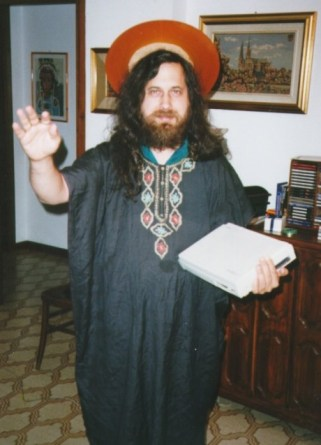
\includegraphics[scale=0.35]{img/saintignucius.jpg}
			\end{figure}		
	\end{columns}

\end{frame}

%------------------------------------------------

\section{90's}

\begin{frame}
    \centerline{1990: Z shell A.K.A. zsh}
\end{frame}

\begin{frame}
	\frametitle{ 90's}
	\textbf{1990: Z shell A.K.A. zsh}\pause
	\begin{itemize}
		\item /bin/bash compatibility, drop-in replacement for Bash.\pause
		\item Most closely resembles Korn shell.\pause
		\item "new" (despite being over 20 years old).\pause
		\item The awesome stuff we'll talk about now.\pause
	\end{itemize}
\end{frame}

%------------------------------------------------

\section{Why use zsh?}

\begin{frame}
    \centerline{First, a reason that's impossible...}
\end{frame}

\begin{frame}
	\centerline{If you're using Mac OS X...}
\end{frame}

\begin{frame}
    \centerline{...your Bash is \textit{old!}}
    	\begin{figure}[h!]
			\adjincludegraphics[width=0.8\linewidth,valign=t]{img/mac.jpeg}
		\end{figure}	
\end{frame}

\begin{frame}
    \centerline{zsh vs bash}
\end{frame}

\begin{frame}
	\frametitle{ The fight!}
	\textbf{zsh vs bash}\pause
	\begin{itemize}
		\item autocomplete\pause
		\begin{itemize}
			\item cd\pause
			\item git\pause
			\item and other..\pause
		\end{itemize}
		\item path expansion\pause
		\item path replacement\pause
		\item string replacement\pause
		\item spelling correction\pause
		\item aliases\pause
		\item programmable file renaming
	\end{itemize}
\end{frame}

\begin{frame}
	\frametitle{ The fight!}
	\textbf{zsh vs bash (2)}\pause
	\begin{itemize}
		\item right prompt\pause
		\item impoved history\pause
		\item shared history between shells\pause
		\item plugin
	\end{itemize}
\end{frame}

\section{The Frameworks}

\begin{frame}
	\frametitle{ The Frameworks!}
	\textbf{Just a little list}\pause
	\begin{itemize}
		\item alf\pause
		\item dotzsh\pause
		\item \huge{oh my zsh}
	\end{itemize}
\end{frame}

\section{Oh My zsh}

\begin{frame}
	\frametitle{ Oh My zsh}
	\textbf{What is?}\pause
	\begin{itemize}
		\item Community-driven framework for managing your zsh configuration\pause
		\item  Includes 200+ optional plugins (rails, git, OSX, hub, capistrano, brew, ant, php, python, etc)\pause
		\item Over 140 themes to spice up your morning\pause
		\item Auto-update tool so that makes it easy to keep up with the latest updates from the community.\pause
		\item http://ohmyz.sh/ or https://github.com/robbyrussell/oh-my-zsh
	\end{itemize}
\end{frame}


\section{Install zsh and oh my zsh}

\begin{frame}
	\frametitle{ Install zsh and oh my zsh}
	\textbf{How?}\pause
	\begin{itemize}
		\item Open Termianl\pause
		\item Install zsh with your package manager (apt-get, pacman, yum, homebrew)\pause
		\item zsh
		\item sudo chsh -s /bin/zsh user (This certainly works on Fedora/Debian/OpenSuse)\pause
		\item For install oh my zsh see the readme.md at: https://github.com/robbyrussell/oh-my-zsh it's very easy\pause
		\item Now you will need to edit the .zshrc file in your home.
	\end{itemize}
\end{frame}

%------------------------------------------------

\begin{frame}
    \centerline{Material:}
    \centerline{https://github.com/paranoiasystem/LinuxDay2015}
\end{frame}

\begin{frame}
    \centerline{The End, Question?}
\end{frame}

%------------------------------------------------

\end{document} 
\grid
